% =============================================================================
% Projektbericht – Konzepte von Programmiersprachen
% Raytracer-Optimierung, SS 2026
% Hochschule Karlsruhe (HKA)
% =============================================================================
\documentclass[11pt, a4paper]{article}

% --- Pakete ---
\usepackage[ngerman]{babel}
\usepackage[utf8]{inputenc}
\usepackage[T1]{fontenc}
\usepackage{lmodern}
\usepackage[left=2.5cm, right=2.5cm, top=2.5cm, bottom=2.5cm]{geometry}
\usepackage{graphicx}
\usepackage{xcolor}
\usepackage{hyperref}
\usepackage{tabularx}
\usepackage{booktabs}
\usepackage{float}
\usepackage{fancyhdr}
\usepackage{titlesec}
\usepackage{parskip}
\usepackage{listings}
\usepackage{siunitx}
\usepackage{amsmath}

% --- Farben (HKA Corporate) ---
\definecolor{hkared}{RGB}{198, 42, 18}
\definecolor{hkagray}{RGB}{100, 100, 100}
\definecolor{codebg}{RGB}{245, 245, 245}
\definecolor{codegreen}{RGB}{0, 128, 0}
\definecolor{codegray}{RGB}{120, 120, 120}
\definecolor{codeblue}{RGB}{0, 0, 180}

% --- Hyperref Setup ---
\hypersetup{
    colorlinks=true,
    linkcolor=hkared,
    urlcolor=hkared,
    citecolor=hkared
}

% --- Section Styling ---
\titleformat{\section}{\large\bfseries\color{hkared}}{\thesection}{1em}{}
\titleformat{\subsection}{\normalsize\bfseries\color{hkared}}{\thesubsection}{1em}{}
\titlespacing*{\section}{0pt}{1.2em}{0.5em}
\titlespacing*{\subsection}{0pt}{0.8em}{0.3em}

% --- Code Listing Style ---
\lstset{
    language=C++,
    backgroundcolor=\color{codebg},
    basicstyle=\ttfamily\footnotesize,
    keywordstyle=\color{codeblue}\bfseries,
    commentstyle=\color{codegreen},
    stringstyle=\color{hkared},
    numberstyle=\tiny\color{codegray},
    numbers=left,
    numbersep=8pt,
    frame=single,
    rulecolor=\color{codegray},
    breaklines=true,
    breakatwhitespace=true,
    tabsize=4,
    showstringspaces=false,
    captionpos=b,
    aboveskip=1em,
    belowskip=1em
}

% --- Header/Footer ---
\pagestyle{fancy}
\fancyhf{}
\fancyhead[L]{\small\color{hkagray}Projektbericht -- Raytracer-Optimierung}
\fancyhead[R]{\small\color{hkagray}KvP, SS~2026}
\fancyfoot[C]{\small\color{hkagray}\thepage}
\renewcommand{\headrulewidth}{0.4pt}

% --- siunitx Setup ---
\sisetup{
    group-separator={.},
    output-decimal-marker={,},
    table-format=6.0
}

% =============================================================================
\begin{document}

% --- Titelseite ---
\begin{titlepage}
    \centering
    
\includegraphics[width=0.35\textwidth]{HKA.jpg}

    {\normalsize\color{hkagray} University of Applied Sciences}\\[0.125cm]
    {\small\color{hkagray} Fakultät für Informatik und Wirtschaftsinformatik}

    \vspace{.5cm}
    {\color{hkared}\rule{\textwidth}{1.5pt}}

    \vspace{1.5cm}
    {\fontsize{24}{30}\selectfont\bfseries\color{hkared} Raytracer-Optimierung}\\[0.6cm]
    {\Large Whitted-Style Raytracer mit Badouel \& Möller-Trumbore}\\[.75cm]
    {\LARGE\bfseries Projektbericht}

    \vspace{.5cm}
    {\large Konzepte von Programmiersprachen}\\[0.3cm]
    {\large Sommersemester 2026}

    \vspace{.5cm}
    {\color{hkared}\rule{0.6\textwidth}{0.5pt}}
    \vspace{1.5cm}

    {\normalsize
    \begin{tabular}{rl}
        \textbf{Betreuer:}  & Prof.~Dr.~Christian~Pape \\[0.5cm]
        \textbf{Autor:}     & Erlind Sejdiu \\[0.5cm]
        \textbf{Abgabe:}    & 29.~April~2026 \\
    \end{tabular}
    }

    \vfill
    {\small\color{hkagray} Version 1.0 -- Stand: \today}
\end{titlepage}

% --- Inhaltsverzeichnis ---
\tableofcontents
\newpage

% =============================================================================
\section{Einleitung}
% =============================================================================

Gegenstand dieses Projektberichts ist die schrittweise Implementierung und Optimierung eines einfachen Raytracers im Rahmen der Veranstaltung \textit{Konzepte von Programmiersprachen}. Der Raytracer wurde in C++17 unter Verwendung der Mathematikbibliothek GLM entwickelt und mit dem GCC-Compiler über CMake übersetzt. Als Testszene dient die bereitgestellte Wavefront-Datei \texttt{teapot\_n\_glass.obj}, die eine Teekanne mit Glasobjekt umfasst und insgesamt 18\,032 Dreiecke enthält. Alle Zeitmessungen beziehen sich auf diese Szene bei einer festen Auflösung von $500 \times 500$ Bildpunkten, um über die Teilaufgaben hinweg vergleichbare Ergebnisse zu erzielen.

Der Bericht dokumentiert die Ergebnisse aller Teilaufgaben. Jeder Abschnitt beschreibt die gewählte Vorgehensweise, die wesentlichen Implementierungsdetails sowie die gemessenen Renderzeiten.

% =============================================================================
\section{Aufgabe 1: Whitted-Style Raytracer mit Brute-Force-Suche}
% =============================================================================

% -----------------------------------------------------------------------------
\subsection{Architektur und Modulstruktur}
% -----------------------------------------------------------------------------

Das Programm ist in vier logische Module unterteilt, die jeweils als eigene Header- bzw. Quelldatei organisiert sind. Das Modul \texttt{Ray} definiert die grundlegende Datenstruktur eines Sehstrahls, bestehend aus einem Ursprungspunkt und einem normalisierten Richtungsvektor. Das Modul \texttt{Camera} kapselt die Kameralogik und berechnet aus einer gegebenen Position, einem Blickpunkt, einem Up-Vektor sowie einem vertikalen Öffnungswinkel das lokale Koordinatensystem der Kamera. Für jeden Bildpunkt kann daraus ein Primärstrahl erzeugt werden, indem die normalisierten Bildkoordinaten $(u, v)$ auf die Bildebene im Weltkoordinatensystem abgebildet werden.

Das Modul \texttt{Mesh} ist für das Einlesen der Szenengeometrie aus dem Wavefront-OBJ-Format zuständig. Es parst die Datei zeilenweise und extrahiert Vertex-Positionen (Zeilen mit Präfix \texttt{v}) sowie Dreiecksdefinitionen (Zeilen mit Präfix \texttt{f}). Da das OBJ-Format Vertex-Indizes in der Form \texttt{v/vt/vn} kodiert, wird lediglich der erste Index bis zum Schrägstrich extrahiert. Die resultierenden Dreiecke werden in einer flachen Liste von \texttt{Triangle}-Strukturen gespeichert, wobei jedes Dreieck durch seine drei Eckpunkte \texttt{v0}, \texttt{v1} und \texttt{v2} repräsentiert wird.

Das Modul \texttt{Intersector} enthält die statische Methode zur Schnittpunktberechnung, deren Implementierung im folgenden Abschnitt erläutert wird.

\newpage
% -----------------------------------------------------------------------------
\subsection{Badouel-Algorithmus (Baseline)}
% -----------------------------------------------------------------------------

Als Baseline für die Schnittpunktberechnung zwischen einem Sehstrahl und einem Dreieck wurde der Algorithmus nach Badouel implementiert. Dieser Algorithmus berechnet zunächst explizit die Ebenengleichung des Dreiecks und den potenziellen 3D-Schnittpunkt des Strahls mit dieser Ebene. 

Um den anschließenden \textit{Point-in-Polygon}-Test durchzuführen, projiziert das Verfahren den 3D-Schnittpunkt und die Dreieckseckpunkte auf eine 2D-Ebene. Dies geschieht durch das simple Weglassen derjenigen Koordinatenachse, bei der die Flächennormale ihre betragsmäßig größte Ausdehnung besitzt (die sogenannte dominierende Achse). Durch diese Projektion auf die xy-, xz- oder yz-Ebene reduziert sich der Test auf das Lösen eines 2D-Gleichungssystems zur Bestimmung der baryzentrischen Koordinaten. Obwohl dieser Ansatz durch die Reduktion auf zwei Dimensionen prinzipiell Multiplikationen einspart, bildet er aufgrund des Branching-Overheads (zur Bestimmung der dominierenden Achse) sowie der initialen Ebenenberechnungen unsere Performance-Baseline.

% -----------------------------------------------------------------------------
\subsection{Möller-Trumbore-Algorithmus (1. Optimierung)}
% -----------------------------------------------------------------------------

Als erste Optimierungsmaßnahme gegenüber der Badouel-Baseline wurde zusätzlich der Möller-Trumbore-Algorithmus implementiert. Dieser bietet gegenüber klassischen Verfahren einen entscheidenden Effizienzvorteil: Er berechnet die baryzentrischen Koordinaten $(u, v)$ direkt im 3D-Raum und vermeidet so die explizite Konstruktion der Dreiecksebene sowie die teuren Fallunterscheidungen für die 2D-Projektion.

Der Algorithmus beruht auf der Umformung der Strahlgleichung $\mathbf{O} + t \cdot \mathbf{D} = (1 - u - v) \cdot \mathbf{V_0} + u \cdot \mathbf{V_1} + v \cdot \mathbf{V_2}$ in ein lineares Gleichungssystem, das mit der Cramerschen Regel gelöst wird. Dabei werden die Kanten $\mathbf{e_1} = \mathbf{V_1} - \mathbf{V_0}$ und $\mathbf{e_2} = \mathbf{V_2} - \mathbf{V_0}$ berechnet, und über Kreuzprodukte und Skalarprodukte die Parameter $t$, $u$ und $v$ bestimmt. Ein Treffer liegt genau dann vor, wenn $u \geq 0$, $v \geq 0$, $u + v \leq 1$ und $t > \varepsilon$ gilt. Der Schwellwert $\varepsilon = 10^{-7}$ verhindert numerische Artefakte bei nahezu parallelen Strahlen.

Die zentrale Implementierung stellt sich wie folgt dar:

\noindent\begin{minipage}{\textwidth}
\begin{lstlisting}[caption={Möller-Trumbore-Schnittpunkttest}]
Intersection Intersector::intersectRayTriangle(
    const Ray& ray,
    const glm::vec3& v0, const glm::vec3& v1, const glm::vec3& v2)
{
    Intersection result = {false, 0.0f, 0.0f, 0.0f};

    glm::vec3 edge1 = v1 - v0;
    glm::vec3 edge2 = v2 - v0;
    glm::vec3 h = glm::cross(ray.direction, edge2);
    float a = glm::dot(edge1, h);

    constexpr float EPSILON = 0.0000001f;
    if (a > -EPSILON && a < EPSILON)
        return result;

    float f = 1.0f / a;
    glm::vec3 s = ray.origin - v0;
    result.u = f * glm::dot(s, h);
    if (result.u < 0.0f || result.u > 1.0f)
        return result;

    glm::vec3 q = glm::cross(s, edge1);
    result.v = f * glm::dot(ray.direction, q);
    if (result.v < 0.0f || result.u + result.v > 1.0f)
        return result;

    result.t = f * glm::dot(edge2, q);
    if (result.t > EPSILON) {
        result.hit = true;
    }
    return result;
}
\end{lstlisting}
\end{minipage}

Der Algorithmus nutzt ein frühzeitiges Abbruchverfahren (Early Rejection): Sobald einer der baryzentrischen Parameter außerhalb des gültigen Bereichs liegt, wird die Berechnung sofort abgebrochen, ohne die verbleibenden Skalarprodukte auszuwerten. Dies reduziert den Rechenaufwand für die Mehrheit der Strahlen, die ein gegebenes Dreieck verfehlen.

% -----------------------------------------------------------------------------
\subsection{Brute-Force-Schnittpunktsuche}
% -----------------------------------------------------------------------------

Da in dieser ersten Teilaufgabe noch keine Beschleunigungsdatenstruktur vorliegt, erfolgt die Bestimmung des nächstgelegenen Schnittpunktes durch eine vollständige lineare Suche über alle 18\,032 Dreiecke der Szene. Für jeden Primärstrahl wird die \texttt{intersectRayTriangle}-Methode auf jedes einzelne Dreieck angewendet und der Treffer mit dem kleinsten $t$-Wert gespeichert. Bei einer Bildauflösung von $500 \times 500$ Pixeln und einem zusätzlichen Schattenstrahl pro beleuchtetem Pixel ergibt sich eine Gesamtzahl von bis zu $500 \times 500 \times 2 \times 18\,032 = 9{,}016 \cdot 10^9$ Schnittpunkttests im ungünstigsten Fall.

% -----------------------------------------------------------------------------
\subsection{Beleuchtung und Schatten}
% -----------------------------------------------------------------------------

Zur Erzeugung eines plastischen Eindrucks wurde ein einfaches Beleuchtungsmodell implementiert. Es besteht aus einer einzelnen Punktlichtquelle an der Position $(5, 10, 5)$ im Weltkoordinatensystem. Trifft ein Primärstrahl auf ein Dreieck, wird zunächst der exakte Auftreffpunkt $\mathbf{P} = \mathbf{O} + t \cdot \mathbf{D}$ berechnet. Die Oberflächennormale ergibt sich aus dem normalisierten Kreuzprodukt der Dreieckskanten.

Für die Schattenberechnung wird ein sekundärer Strahl (Shadow Ray) vom Auftreffpunkt in Richtung der Lichtquelle ausgesendet. Der Startpunkt wird dabei um einen kleinen Offset in Normalenrichtung ($0{,}001$) verschoben, um das Phänomen der Shadow Acne zu vermeiden, bei dem ein Dreieck sich selbst fälschlicherweise verschattet. Trifft der Schattenstrahl auf seinem Weg ein Objekt, dessen Entfernung kleiner ist als die Distanz zur Lichtquelle, wird der Punkt als verschattet deklariert und lediglich mit einem schwachen Umgebungslicht dargestellt. Andernfalls wird die Helligkeit nach dem Lambertschen Beleuchtungsmodell berechnet, bei dem der Kosinus des Einfallswinkels zwischen Lichtrichtung und Oberflächennormale die Intensität bestimmt:

\begin{lstlisting}[caption={Schattenstrahl mit Distanzprüfung}]
float distanceToLight = glm::length(lightPos - hitPoint);
Ray shadowRay = {hitPoint + normal * 0.001f, lightDir};
Intersection shadowIsect;
Triangle dummyTriangle;
bool inShadow = findClosestHit(shadowRay, scene.triangles,
                               shadowIsect, dummyTriangle);

// Nur Objekte ZWISCHEN Trefferpunkt und Lichtquelle erzeugen Schatten
if (inShadow && shadowIsect.t > distanceToLight) {
    inShadow = false;
}
\end{lstlisting}

Die Distanzprüfung in Zeile 9--11 stellt sicher, dass ausschließlich Objekte, die sich tatsächlich zwischen dem Auftreffpunkt und der Lichtquelle befinden, einen Schatten werfen. Ohne diese Prüfung könnten Objekte hinter der Lichtquelle fälschlicherweise als Okkluder erkannt werden.

% -----------------------------------------------------------------------------
\subsection{Zeitmessung}
\label{sec:zeitmessung}
% -----------------------------------------------------------------------------

Die Zeitmessung erfolgt über \texttt{std::chrono::high\_resolution\_clock} und umfasst ausschließlich den Render-Loop ohne die Ladezeit der Szene. Gemessen wurde auf einem System mit Ubuntu unter WSL. Die folgende Tabelle zeigt die Renderzeiten für die Brute-Force-Implementierung (500\,$\times$\,500 Pixel, 18\,032 Dreiecke).

\begin{table}[H]
    \centering
    \caption{Renderzeiten der Brute-Force-Implementierung (500\,\times\,500 Pixel, 18\,032 Dreiecke)}
    \label{tab:zeiten-aufgabe1}
    \begin{tabular}{l S[table-format=6.0] S[table-format=6.0]}
        \toprule
        \textbf{Konfiguration} & {\textbf{Badouel [ms]}} & {\textbf{Möller-Trumbore [ms]}} \\
        \midrule
        Release (mit \texttt{-O3 -march=native})    & 100067 &  65019 \\
        \bottomrule
    \end{tabular}
\end{table}

Die Messergebnisse zeigen die Ausführungszeiten im vollständig optimierten Release-Modus (Compiler-Flags \texttt{-O3 -march=native}). Es zeigt sich, dass der Möller-Trumbore-Algorithmus unsere Baseline (Badouel) durch Reduktion von Branching und Verzicht auf Ebenenkonstruktion messbar schlägt. Der Geschwindigkeitsvorteil beträgt hierbei etwa den Faktor $1,5\times$.

Trotz des Einsatzes des performanteren Algorithmus bleibt die absolute Renderzeit mit rund 100 Sekunden (Badouel) bzw. 65 Sekunden (Möller-Trumbore) sehr hoch. Die Ursache liegt in der linearen Komplexität $\mathcal{O}(n)$ der Brute-Force-Suche pro Strahl, wobei $n$ die Anzahl der Dreiecke in der Szene bezeichnet. Dies motiviert die Einführung einer hierarchischen Beschleunigungsdatenstruktur in der nachfolgenden Aufgabe.

% =============================================================================
\section{Aufgabe 2: Beschleunigungsdatenstruktur}
% =============================================================================

\textit{Dieser Abschnitt wird nach Implementierung des k-d-Baums mit Slab-Test und Median-Unter\-teilung ergänzt.}

% =============================================================================
\section{Aufgabe 3: AVX-Optimierung mit Packet Tracing}
% =============================================================================

\textit{Dieser Abschnitt wird nach Implementierung der AVX-basierten Parallelisierung ergänzt.}

% =============================================================================
\section{Zusammenfassung und Ausblick}
% =============================================================================

\begin{table}[H]
    \centering
    \caption{Gesamtübersicht der Renderzeiten im Release-Modus}
    \label{tab:zeiten-gesamt}
    \begin{tabular}{l S[table-format=6.0] S[table-format=3.1]}
        \toprule
        \textbf{Implementierungsschritt} & {\textbf{Renderzeit [ms]}} & {\textbf{Speedup}} \\
        \midrule
        Aufgabe 1: Brute-Force (Badouel) & 100067 & {1,0\times} \\
        Aufgabe 1: Brute-Force (M.-T.)   &  65019 & {1,5\times} \\
        Aufgabe 2: k-d-Baum              & {--}   & {--} \\
        Aufgabe 3: AVX Packet Tracing    & {--}   & {--} \\
        \bottomrule
    \end{tabular}
\end{table}

Die bisherige Implementierung stellt eine funktionsfähige Basislinie dar. Der Badouel-Algorithmus fungiert dabei als Referenz für die Bewertung zukünftiger Optimierungen, beginnend mit dem ersten Speedup durch Möller-Trumbore. In den folgenden Aufgaben wird zunächst die algorithmische Komplexität durch einen k-d-Baum weiter reduziert und anschließend durch SIMD-Parallelisierung mittels AVX-Instruktionen die Hardwareausnutzung verbessert.

\begin{figure}[H]
    \centering
    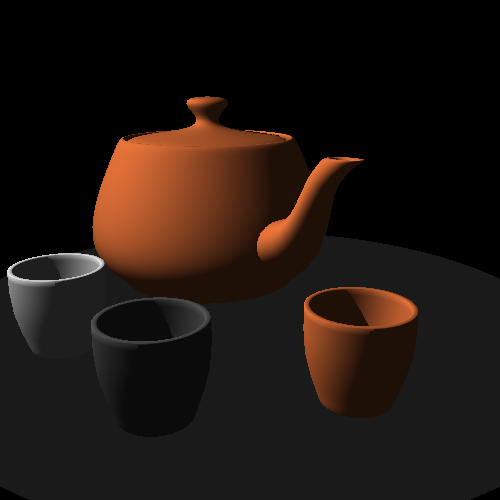
\includegraphics[width=0.7\textwidth]{../build-release/output.png}
    \caption{Gerendertes Ergebnis der Szene (Teekanne und Glasobjekt) mit einfachem Schatten}
    \label{fig:render_output}
\end{figure}

\end{document}
